\documentclass[10pt,a4paper]{article}
\usepackage[lutf8]{inputenc}
\usepackage[french]{babel}
\usepackage[T1]{fontenc}
\usepackage{lmodern}
\usepackage{amsmath}
\usepackage{amsfonts}
\usepackage{amssymb}
\usepackage{graphicx}
\usepackage[top = 2.5 cm, bottom = 2.5 cm, left = 2.5 cm, right = 2.5 cm]{geometry}
\usepackage{listings}

\author{Philippe Verbist  Antoine Paris\\3521-13-00 \ \ \ \ 3158-13-00}
\title{DJ'Oz : Rapport de projet}
\date{4 décembre 2014}
\begin{document}
\maketitle


\section{Structure du programme}
Nous avons divisé, comme demandé, le programme en trois parties:
\begin{itemize}
	\item Une fonction Interprete, qui prends une partition en 	paramètre et qui renvoie une liste d'échantillons;
	\item une fonction Mix, qui prend (1) une fonction qui permet d'interpréter une partition  et (2) une musique et qui renvoie un vecteur audio, sous la forme d'une liste de flottants compris dans l'intervalle [-1.0;1.0];
	\item un fichier example.dj.oz, qui contient une musique.
\end{itemize}



	\begin{table}[ht!]
		\centering
			\begin{tabular}{|p{0.15\textwidth}|p{0.22\textwidth}|p{0.25\textwidth}|p{0.25\textwidth}|}
			\hline
			\textbf{Fonction}		& \textbf{Sous-fonction maitresse}& \textbf{Sous-fonctions principales} & \textbf{Autres sous-fonctions}	\\
			\hline
Interprete		&InterpreteFlattened	& DureeTrans, Etirer, Bourdon, Transpose, Instrument, ... & ToNote, NumberOfSemiTones, ...\\
			\hline
Mix 	& MixMusic &  MixVoice, Merge, RepetitionNB, Echo, ... &  Fill, Combine, ...\\
			\hline 


			\hline
			\end{tabular}
		\caption{Résumé des fonctions de notre programme.}
	\end{table}


\section{Décisions prises et astuces de programmation}
\paragraph{Programmation déclarative} Aucune structure non-déclarative n'a été nécessaire pour écrire notre programme. Nous n'en avons donc pas utilisé.

\paragraph{Récursion terminale}
Pour rendre notre code plus rapide, nous nous sommes arrangés pour que toutes nos sous-fonctions
 soient récursives terminales. Pour ce faire, nous avons, notamment, utilisé des accumulateurs.
 
 \paragraph{Privilégier autant que possible l'appel de fonctions déjà créées} Une des grandes difficultés de ce projet était l'"encapsulation" de données dans d'autres données. Par exemple, une musique peut contenir un filtre qui contient un filtre qui contient un merge qui contient une musique qui contient une partition qui contient une transformation, ... Pour pouvoir faire sortir progressivement tout ces niveaux de données, nous avons dû systématiquement, dans chaque sous-fonction secondaire, ré-appeler la fonction maitresse.

\paragraph{Astuce lors des récursions}
A de nombreux endroits du code, nous devions construire progressivement une liste. Une technique (lorsque l'on utilise un accumulateur) consiste à utiliser la fonction \{Append Accumulateur NouvelElement\}. Le problème est que Append va d'abord parcourir l'accumulateur en entier avant "d'ajouter" le nouvel élément... Or, très souvent, l'accumulateur est très grand (en particulier si la musique à mixer est grande) et le nouvel élément très petit (il s'agit, très souvent, d'un seul élément). Pour accélérer notre code, nous avons donc inversé les arguments: \{Append NouvelElement Accumulateur\}, et à la fin de la fonction, nous renvoyons \{Reverse Accumulateur\}. Ceci permet de ne parcourir qu'une seule fois l'accumulateur en entier, et donc de réduire la complexité temporelle de la fonction de O(n!) à O(n). Cette technique s'est avérée particulièrement efficace lorsque nous devions construire un vecteur audio d'une certaine fréquence (fonction Fill), dont la longueur moyenne est de 44 100 éléments (1 seconde)

\paragraph{Astuce lors de Reverse} Cependant, l'astuce précédente, bien qu'elle permettre d'accélérer grandement nos fonctions, a amené un autre problème: si NouvelElement est une liste, alors non seulement les éléments ne seront plus dans l'ordre, mais en plus il sera impossible de les reclasser dans le bon ordre en appelant \{Reverse Acc\}. Pour corriger ce problème, nous créons une liste de listes (voir Figure \ref{fig:astuceReverse}), et on renvoie la liste en utilisant \{Flatten \{Reverse Acc\}\}.

\begin{figure}[h!]
\centering
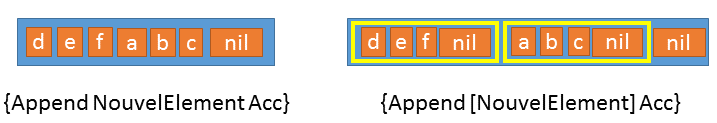
\includegraphics[width=10cm]{images/AstuceAppend.png}
\caption{A gauche: une liste impossible à reclasser dans le bon ordre. A droite: une liste de listes qu'il est possible de reclasser dans le bon ordre en appelant Reverse.}
\label{fig:astuceReverse}
\end{figure}





\section{Complexité calculatoire}
Comme nos fonctions peuvent Dans cette section, nous donnons les complexité calculatoire
propre de chaque fonction, c'est à dire sans tenir des sous-fonctions
utilisées.

	\begin{table}[ht!]
		\centering
			\begin{tabular}{|p{0.40\textwidth}|p{0.25\textwidth}|p{0.25\textwidth}|}
			\hline
			\textbf{Fonctions}																& \textbf{Temporelle}							& \textbf{Spatiale}	\\
			\hline
			InterpreteFlattened																& $n$ 														& $1$ \\
			\hline
			DureeTrans WantedDuration Part 										& $n$, taille de Part							& $1$ \\
			\hline 
			Etirer Facteur Part																& $n$, taille de Part 						& $1$ \\
			\hline
			Bourdon Note Part																	& $n$, taille de Part 						& $1$ \\
			\hline
			Transpose Demitons Part														& $n$, taille de Part 						& $1$ \\
			\hline
			Instrument InstrumentAtom Part										& $n$, taille de Part							& $1$ \\
			\hline
			VoiceDuration ListEchantillon											& $n$, taille de ListEchantillon	& $1$ \\
			\hline
			NumberOfSemiTones Note														& $1$ 														& $1$ \\
			\hline
			NameToNumber Name																	& $1$ 														& $1$ \\
			\hline
			ToNote Note																				& $1$ 														& $1$ \\ 
			\hline
			\hline
			MixMusic Music																		& $n$, taille de Music						& $1$ \\
			\hline
			MixVoice Voice																		& $n$, taille de Voice						& $1$ \\
			\hline
			Fill F Duree																			& $n$, valeur de Duree						& $1$ \\
			\hline
			Merge MusicsWithIntensity													& $n$, taille de MusicsWithIntensity	& $1$ \\
			\hline
			Combine L1 L2																			& $n$, taille de la plus grande des listes	& $1$ \\
			\hline
			Lissage AV Duree																	& $n$, taille de AV								& $1$ \\
			\hline
			HauteurToNote																			& $1$ 														& $1$ \\
			\hline
			NumberToNote																			& $1$ 														& $1$ \\
			\hline
			\end{tabular}
		\caption{Analyse de la complexité calculatoire de nos fonctions.}
	\end{table}


\section{Extensions}



\section{Pistes d'améliorations}
% TODO : gestion des erreurs


\newpage



\subsection{Fonction Interprete}
\subsubsection{Sous-fonction principale}
Cette fonction est codée autour de la sous-fonction fun {InterpreteFlattened FlattenedPartition},
 qui parcourt la partition passée en paramètre et qui, à chaque itération, prend le premier
élément de la liste, l'analyse (dans l'ordre: s'agit-il d'une transformation, d'un silence ou d'une note?)
 et crée un échantillon. Cet échantillon est soit obtenu immédiatement s'il s'agit d'une note ou d'un
silence (cas simple), soit après l'appel d'une autre sous-fonction s'il s'agit d'une transformation -
chaque transformation ayant une fonction qui lui correspond (cas complexe). Par exemple, la sous-fonctioN
{Etirer Facteur Part} est appelée pour la transformation etirer(facteur:F P). Ceci est vrai pour toutes
les transformations, sauf muet(P), pour laquelle il n'existe pas de sous-fonction {Muet Part}.

\subsubsection{Sous-fonctions de transformation}
Comme dit ci-dessus, il y a autant de fonctions de transformation que de transformations (sauf pour muet(P)). 
On retrouve donc :
\begin{itemize}
	\item \begin{verbatim} {WantedDuration Part} \end{verbatim}
	\item \begin{verbatim} {Etirer Facteur Part} \end{verbatim}
	\item \begin{verbatim} {Bourdon Note Part} \end{verbatim}
	\item \begin{verbatim} {Transpose Demitons Part} \end{verbatim}
	\item \begin{verbatim} {Instrument InstrumentAtom Part} \end{verbatim} 
\end{itemize}

Le fonctionnement  de chacune de ces sous-fonctions suit toujours le même schéma :
\begin{itemize}
	\item la partition passée en paramètre \verb Part  est transformée en une liste d'échantillon 
				par un appel à \begin{verbatim} {InterpreteFlattend Partition} \end{verbatim} (la sous-fonction principale)
	\item cette liste d'échantillons est ensuite parcourue par une sous-sous-fonction, qui applique 
				la transformation demandée sur chacun des échantillons.
\end{itemize} 

Mettre un exemple?

\subsubsection{Sous-fonctions complémentaires}
Pour alléger certaines tâches de nos sous-fonctions de transformation,  nous avons créé 4 sous-fonctions complémentaires, à savoir:
\begin{itemize}
	\item {VoiceDuration ListEchantillon}
	\item {NumberOfSemiTones Note}
	\item {NameToNumber Name}
	\item {ToNote Note}\footnote{Cette fonction nous a été donnée dans l'énonce du projet. Elle a été reprise sans être modifiée.}
\end{itemize}

La seule fonction qui présente ici un réel intérêt est la fonction {NumberOfSemiTones Note}. Nous l'expliquerons un peu plus loin.

\subsection{Fonction Mix}
\subsubsection{Sous-fonction principale}
A l'instar de la fonction Interprete, Mix est codée autour d'une sous-fonction principale: 
fun {MixMusic Music}, qui parcourt la musique (une liste de morceaux) passée en paramètre 
et qui, à chaque itération, prend le premier élément de la liste, l'analyse d'après toutes
 les possibilités que peut être un morceau et crée un vecteur audio. 
De nouveau, deux cas se distinguent :
\begin{itemize}
	\item un cas simple: le vecteur audio peut être obtenu directement à partir d'une voix, 
				d'une partition ou d'un vecteur audio déjà existant dans un fichier .wav.
	\item un cas plus complexe, à savoir un filtre ou un merge (jouer deux musiques en même temps),
				qui s'applique sur un vecteur audio déjà existant. Nous appelons ces cas 'complexes' car ils 
				peuvent chacun s'appliquer sur un nouveau morceau, qui peut lui-même être soit simple soit complexe.
				Il est en effet permis d'appliquer un filtre sur un filtre sur un filtre... A noter que l'extrémité 
				d'une telle chaine est toujours un cas simple.
\end{itemize}

\subsubsection{Sous-fonctions de création de vecteur audio (cas simples)}
Les 3 cas simples cités ci-dessus (voix, partition, wave)  ne nécessitent que l'utilisation
de deux sous-fonctions (voix et partition reviennent au même, puisqu'il suffit d'appliquer Interprete sur partition()) :
\begin{itemize}
	\item {MixVoice Voice} (dont la méthode est donnée dans le rapport)
	\item {Projet.readFile File} (fonction donnée)
\end{itemize}

\subsubsection{Sous-fonctions de filtre et merge (cas complexes)}
Il y a autant de sous-fonction de filtre qu'il y a de filtres possibles (sauf pour renverser):
\begin{itemize}
	\item  {RepetitionNB NB AV}
	\item {RepetitionDuree Duree AV}
	\item {Clip Bas Haut AV}
	\item ... (la suite de la liste se déduit assez facilement, et n'est pas particulièrement intéressante)
\end{itemize}


\end{document}